\documentclass[11pt]{article}
\RequirePackage{fullpage}
%\RequirePackage[font=small,labelfont=bf]{caption}
\RequirePackage{amsmath,amssymb,amsthm}
\RequirePackage{graphicx}
\RequirePackage[hidelinks]{hyperref}
\RequirePackage{subcaption}
\RequirePackage{wasysym}
\RequirePackage{authblk}
\RequirePackage{bm}
\RequirePackage{bbm}
%\RequirePackage[osf]{mathpazo}
\let\temp\rmdefault
\RequirePackage{mathpazo}
\let\rmdefault\temp

\RequirePackage[bibstyle=authoryear,citestyle=authoryear-comp,
                date=year,
                maxbibnames=9,maxnames=5,maxcitenames=2,
                backend=biber,uniquelist=false,uniquename=false,
                % style=apa,
                sorting=nyt,
                % sorting=,
                hyperref=true]{biblatex}
\usepackage{color}
\usepackage{nicefrac}


% line numbers:
\RequirePackage{lineno}
%\modulolinenumbers[5]
\renewcommand\linenumberfont{\normalfont\tiny\sffamily\color{black}}

\renewcommand{\P}{\mathbb{P}}
\newcommand{\E}{\mathbb{E}}
\newcommand{\V}{\text{V}}
\DeclareMathOperator{\var}{var}
\DeclareMathOperator{\cov}{cov}

\addbibresource{biblio.bib}

\title{Supplementary Materials}

\author{Vince Buffalo and Andrew Kern}

\begin{document}
\maketitle

\section{Human Genomic Data}

\subsection{YRI Samples}

In order to try to ensure accurate estimation of pairwise diversity, which is a
ratio estimator that is sensitivity to its denominator, we use the complete
per-basepair genotype calls (gVCF) produced by Illumina's DRAGEN pipeline
\parencite{Illumina_Inc2020-dk}. The original samples were from 178 Yoruban
individuals sequenced to 30x by the New York Genome Center
\parencite{Byrska-Bishop2022-tn}. This allows for filtering to be applied to
the entire genome at once, rather than just variants, so the denominator does
not need to be estimated separately.

The full list of samples is available in TSV format in the GitHub repository
(\path{data/h1kg/yri_samples.tsv}).

\subsection{Filtering gVCFs}

gVCFs were filtered using a custom Python tool, \texttt{gvcf2counts.py} (in
\path{tools/gvcf2counts.py}), which reads the gVCFs, filters them according to
the criteria below, and outputs a Numpy \path{.npy} file of reference and
alternative allele counts for each chromosome (hereafter, ``allele counts
matrices").

Genotypes are included in the allele count if and only if:

\begin{enumerate}
  \item The variant call is set to \texttt{PASS} in the VCF.
  \item The \texttt{QUAL > 50}.
  \item The \texttt{GQ > 30} (or \texttt{RGQ > 30} for invariant sites).
\end{enumerate}

Because the data underlying the counts files are per-basepair resolution gVCFs,
each chromosome's allele counts matrix is of size $l \times 2$, where $l$ is
the total chromosome length. Basepairs that fail these filtering requirements
lead to a row of zero counts, e.g. no observed reference and alternative allele
counts, and thus do not effect the data that goes into the binomial likelihood
or $\pi$ estimates used in figures.

\subsection{Site-based Filtering of Counts}

The allele counts matrices include many basepairs that may have allele counts
that pass the genotype call filters, but are still need to be filtered out
because the region of the genome may produce unreliable estimates. The
following filters are applied based on masking regions:

\begin{enumerate}
  \item \textbf{Non-accessible regions}: masks out centromeres (\texttt{acen} entries in
    \texttt{cytoBand.txt}), with 5Mbp padding on either side. The file of
    passing masks is \path{data/annotation/no_centro.bed}. 

  \item \textbf{Reference masking}: soft and hard-masked regions in the human GRCh38
    reference genome are also masked.

  \item \textbf{Non-``putatively" neutral regions}: Additionally, for fitting our
    likelihood and estimating observed pairwise diversity, we only consider .
    This masks out phastCons regions (from
    \path{phastConsElements100way.bed.gz}) and Ensembl gene regions (from
    annotation file \path{Homo_sapiens.GRCh38.107.chr.gff3.gz}).  While introns
    are possibly under some weak selection, they collectively make up nearly
    40\% of the human genome and are included so genome-wide diversity can be
    estimated more precisely (possibly at the expense of some bias).
\end{enumerate}

These files are all produced by the Snakemake file \path{data/annotation/Snakefile}.

\begin{figure}[!htb]
  \centering
  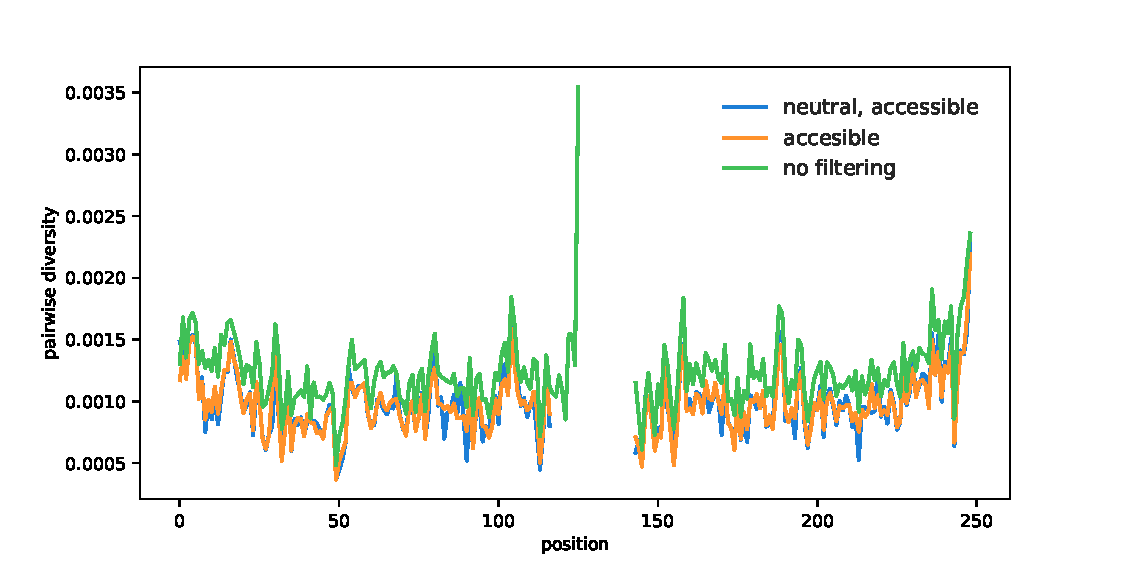
\includegraphics{figures/supplementary/chr1_diversity_filtering.pdf}

  \caption{Estimates of chromosome 1 YRI diversity in non-overlapping megabase
    windows, under different filtering criteria. The filtering criteria are,
    (1) ``neutral, accessible" which includes only putatively neutral sites, and
    ignores regions masked as inaccessible, (2) ``accessible" which is only ignores
  sites masked as inaccessible, and (3) ``no filtering" which uses all available
data. Note that filtering changes the absolute level of diversity, but has more
minor effects on regional patterns of diversity at the megabase scale.}

  \label{suppfig:chr1-diversity}
\end{figure}

\begin{table}
\centering
\begin{tabular}{lrrr}
  \hline
chrom &  accessible &  neutral &  both \\
  \hline
 chr1 &        42.4 &     64.4 &  22.9 \\
 chr2 &        46.8 &     58.7 &  23.7 \\
 chr3 &        44.1 &     62.9 &  24.8 \\
 chr4 &        44.0 &     59.3 &  21.5 \\
 chr5 &        44.1 &     58.0 &  21.4 \\
 chr6 &        45.0 &     58.0 &  22.1 \\
 chr7 &        44.4 &     65.8 &  26.4 \\
 chr8 &        43.8 &     61.2 &  23.1 \\
 chr9 &        39.2 &     64.5 &  20.3 \\
chr10 &        44.6 &     62.8 &  25.3 \\
chr11 &        42.7 &     63.5 &  23.4 \\
chr12 &        41.7 &     62.7 &  22.7 \\
chr13 &        39.7 &     62.0 &  18.3 \\
chr14 &        37.6 &     65.4 &  19.0 \\
chr15 &        37.0 &     69.4 &  20.3 \\
chr16 &        39.4 &     63.8 &  20.9 \\
chr17 &        40.4 &     64.0 &  22.3 \\
chr18 &        40.9 &     59.8 &  19.8 \\
chr19 &        30.9 &     69.8 &  18.0 \\
chr20 &        36.9 &     61.6 &  19.8 \\
chr21 &        31.6 &     68.6 &  18.2 \\
chr22 &        26.9 &     75.0 &  16.4 \\
\end{tabular}
\end{table}

\subsection{Data Summary Matrices}

Our underlying data for all likelihood and pairwise diversity estimates is the
allele count matrix $\mathbf{C}$ with dimensions $L \times 2$, where $L$ is the
chromosome length. This is transformed to a pairwise summary matrix with
identical dimensions, $\mathbf{Y}$. The first column of $\mathbf{Y}$ is the
number of pairwise comparisons between chromosomes that are identical, and the
second column is the number that are different. Both of these columns are
combinatoric summaries of the raw allele counts matrix needed for the binomial
likelihood and pairwise diversity estimates. Let $[c_1, c_2]$ be a row of
$\mathbf{C}$ for basepair $l$ (the $l$ index is omitted for clarity), and $n =
c_1 + c_2$. Then, the (1) total number of pairwise combinations of chromosomes
$n_T$, (2) the number of pairwise with identical alleles $n_S$, and (3) the
number of pairwise combinations with differing alleles $n_D$ are respectively,

\begin{align*}
  n_T &= \frac{n(n-1)}{2} \\
  n_S &= {c_1 \choose 2} + {c_2 \choose 2} \\
  n_D &= n_T - n_S
\end{align*}
%
which would be stored in row $\mathbf{Y}_l = [n_S, n_D]$. Note that the
per-site $\mathbf{Y}$ handles non-polymorphic sites and missing data.
Non-polymorphic sites have $n_S = {n \choose 2}$ and $n_D = 0$, and missing
data has $n_S = n_D = 0$.

\subsection{Pairwise Diversity Estimates}

The pairwise diversity at site $l$ across the $n$ sampled chromosomes can be
calculated from the $\mathbf{Y}$ matrix as follows,

\begin{align}
  \pi(l) = \frac{n_D}{n_T}
\end{align}

which is identical to the more common expression of this estimator, 

\begin{align}
  \pi(l) = \frac{2}{n(n-1)} \sum_{i < j}^n k_{i,j}
\end{align}

where $k_{i,j}$ is 1 if the alleles at this site differ, and 0 otherwise. Note
that for sites with missing data, $c_1 = c_2 = 0$ and thus $n_T = 0$ and the
division is invalid. Such cases were marked as missing with floating point
values \texttt{NaN}s. Binned summaries of data are weighed by the number of
complete cases, e.g. rows with $c_1 + c_2 > 0$.

This per-basepair diversity is then averaged over all callable bases, to give a
genome-wide or window estimate of diversity of accessible bases in the set
$\mathcal{A}$,

\begin{align*}
  \bar{\pi}(\mathcal{A}) = \frac{\sum_{l \in \mathcal{A}} \pi(l)}{L_\mathcal{A}}.
\end{align*}

where $L_\mathcal{A} = |\mathcal{A}|$ is the number of accessible bases. Note
that the sum in the numerator is random over the sample of chromosomes sampled
from the population. Estimates of pairwise diversity often condition on the
accessible bases, and thus treat this as fixed. However, the number of
accessible bases varies across the chromosome; this can lead to a source of
apparent bias during block-bootstrap estimates of uncertainty.  In this case,
pairwise diversity is a ratio estimator, and is thus biased, since by Jensen's
inequality $\E(\nicefrac{y}{x}) \ge \nicefrac{\E(y)}{\E(x)}$ for random
variables $x$ and $y$.

The genome-wide $\bar{\pi}$ can also be estimated by summing the columns of
$\mathbf{Y}$, and calculating $\nicefrac{n_D}{n_T}$.

\subsection{Window-based Summaries and filtering}

\begin{figure}[!htb]
  \centering
  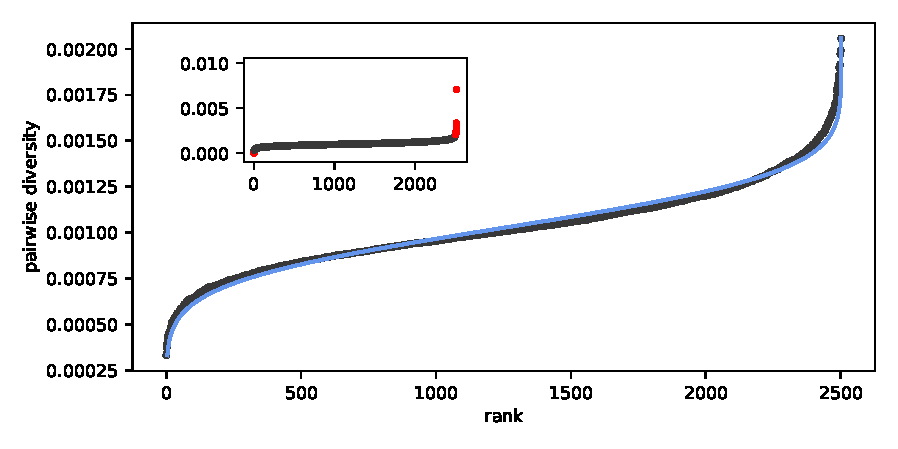
\includegraphics{figures/supplementary/diversity_trimming_dist.pdf}

  \caption{The distribution of diversity across the genome at the megabase
  scale, with outliers trimmed. The blue line is the normal CDF, fit with MLE
parameters XXX. The inset figure is the untrimmed data, with trimmed points
shown in red.}

  \label{suppfig:trimming}
\end{figure}



The likelihood method is fit to non-overlapping binned summaries of the allele
counts matrix. 


Based on exploratory data analyses, some bins were outliers and
excluded (XXX).

\begin{enumerate}
  \item \textbf{Fraction of inaccessible sites per window}.  \path{mask_inaccessible_bins_frac}
  % \item \textbf{Edge truncation}

  \item \textbf{Outliers}: Based on exploratory analysis, there were some
    regions with very high diversity. The 0.05\% right tail was excluded.

\end{enumerate}


% supp data
% - npy files
% - edge trunation

\section*{Likelihood}

Our model is essentially a generalized nonlinear model with a binomial link
function. This is the form used by \textcite{Elyashiv2016-vt} and
\textcite{Murphy2022-sj}. These models fit the observed number of pairwise
nucleotide differences in genomic windows to the expected pairwise diversity
under some evolutionary model. We only consider BGS models here, so the mean
function for position $x$ is the product of the proportion by which BGS reduces
diversity at $x$, $B(x)$, and genome-wide neutral diversity $\pi_0$,

\begin{align}
  \pi(x) = B(x, \Phi) \pi_0
\end{align}

$\Phi$ is the set of BGS parameters (i.e. the DFE for each feature type and
mutation rate), and $\pi_0$ is determined by the drift-effective population
size, set by only reproductive and reproductive processes. Then the ob



fit a nonlinear theoretic equation to
observed count data summarized at some pre-specified scale. 

putatively neutral site, the observed number of pairwise differences at site
$i$ is modeled as,

\begin{align}
  n_{D,i} \sim \text{Binom}(\pi_i, n_{T,i})
\end{align}

use observed count data summarized at
some pre-specified scale 

\begin{align}
  \log\mathcal{L}(\theta) = \sum_{v \in \mathcal{V}} \sum_{i \ne j \in \mathcal{S}} \log(P(O_{i,j}(v) | \theta))
\end{align}

where $\mathcal{V}$ is the set of putatively neutral sites, $\mathcal{S}$ is
the set of samples, and $\theta$ are the BGS parameters. The indicator variable
$O_{i,j}(v)$ is 1 if samples $i$ and $j$ are different at site $v$, and zero
otherwise. Thus as they specify in the paper, 

\begin{align}
  P(O_{i,j}(v) | \theta) = 
    \begin{cases}
      \pi(v | \theta), & O_{i,j}(v) = 1 \\
      1-\pi(v | \theta), & O_{i,j}(v) = 0 \\
    \end{cases}.
\end{align}

The total size of the set of samples $\mathcal{S}$ is $n_\mathcal{S} =
|\mathcal{S}|$. Assuming all sites are biallelic, we can simplify the inner
summation by counting the number of possible same and different pairwise
combinations. If a site $v$'s vector of allele counts is $[c_1, c_2]$, the
total number of pairwise combinations with the same alleles is

\begin{align}
  n_s(v) = {c_1 \choose 2} + {c_2 \choose 2}
\end{align}

and the number of different pairwise combinations is 

\begin{align}
  n_d(v) = n_T - n_s(v)
\end{align}

where $n_T = n_\mathcal{S} (n_\mathcal{S} - 1) / 2$  is the total number of
pairwise combinations across the sample set $\mathcal{S}$. Note that these
site-specific counts allow us to use allelic counts directly, and can vary
across sites. Our log-likelihood is then,

\begin{align}
  \ell(\theta) &= \sum_{v \in \mathcal{V}} \left[\log(\pi(v | \theta)) n_\text{D}(v) + \log(1-\pi(v | \theta)) n_\text{S}(v)\right].
\end{align}

In practice, we calculate these values across bins. For each bin, we treat
$\pi(v | \theta)$ as fixed, assuming that at this scale, the variation in
expected diversity across sites is minimal. For a particular chromosome, we
have two classes of sites: those included in the diversity calculation and
those ignored. The former sites are all putatively neutral and have reliably
called genotypes, and the other sites are possibly non-neutral or do have
reliably called genotypes. The total log-likelihood is the sum of bin likelihoods,
$\ell(b)$

\begin{align}
   \ell(\theta) =  \sum_b \ell(b | \theta)
\end{align}

The likelihood within a bin is then,

\begin{align}
  \ell(b | \theta)  &= \log(\bar{\pi}(b | \theta)) \sum_{v \in \mathcal{V}_b} n_D(v) + \log(1-\bar{\pi}(b | \theta)) \sum_{v \in \mathcal{V}_b} n_S(v)  \\
                               &= \log(\bar{\pi}(b | \theta)) Y_D(b) + \log(1-\bar{\pi}(b | \theta)) Y_S(b)
\end{align}
%
where the two sum terms as $Y_D(b)$ and $Y_S(b)$ are data reductions at the bin
level.

If the data are such that only polymorphic sites are considered, we can adapt
this by partitioning the set $\mathcal{V}$ of neutral sites into polymorphic
($\mathcal{P}$) and fixed sites ($\mathcal{F}$), i.e. $\mathcal{V} =
\mathcal{P} \cup \mathcal{F}$ and $\mathcal{P} \cap \mathcal{F} = \varnothing$.
For all $v \in \mathcal{F}$, $n_d(v) = 0$ and $n_s(v) = n_T$.

Then, 

\begin{align}
  \ell(\theta) &= \sum_{v \in \mathcal{V}} \left[\log(\pi(v | \theta)) n_\text{D}(v) + \log(1-\pi(v | \theta)) n_\text{S}(v)\right] \\
                  &= \sum_{v \in \mathcal{P}} \left[\log(\pi(v | \theta)) n_\text{D}(v) + \log(1-\pi(v | \theta)) n_\text{S}(v)\right] + \sum_{v \in \mathcal{F}} \log(1-\pi(v | \theta)) n_T(v)  \\
\end{align}

\begin{align}
  \ell(b | \theta)  &= \log(\bar{\pi}(b | \theta)) \sum_{v \in \mathcal{P}_b} n_\text{D}(v) + \log(1-\bar{\pi}(b | \theta)) \left(\sum_{v \in \mathcal{P}_b} n_\text{S}(v) +  \sum_{v \in \mathcal{F}_b} n_T(v)  \right).
\end{align}

Note that if we assume that the total number of combinations at each fixed site
is constant, e.g. $n_T = n_T(v)$ for all $v$, then we can use $\sum_v n_T(v) =
n_T |\mathcal{F}_b|$.

\
\section*{The }

The core parts of our likelihood are,

\begin{align}
  \ell(\theta) &=  \sum_b [\log(\bar{\pi}(b | \theta)) Y_D(b) + \log(1-\bar{\pi}(b | \theta)) Y_S(b)]
\end{align}

where,

\begin{align}
  \bar{\pi}(b |\theta) = \pi_0(b) \bar{B}(b | \theta).
\end{align}

Here, $\bar{B}(b | \theta)$ is the predicted reduction in diversity due to BGS
in window $b$, given background selection parameters $\theta$. In practice,
this is site-specific. We can write the reduction at any neutral site $v$ in
the genome as the product of $B$s across all segments, 

\begin{align}
  B(v | \theta) = \exp\left(- \sum_g \int f(\mu(\mathcal{A}(g)), s, S_g) w(s|\mathcal{A}(g)) ds \right)
\end{align}

where $S_g$ is exogenous genomic data about the segment, $S_g = \{L_g, r_g,
\rho(|v-p_g|)\}$, where $L_g$ is the segment's length, $r_g$ is the
recombination rate per basepair in the segment, and $\rho(|v-p_g|)$ is the
recombination distance between the focal site $v$ and the segment position
$p_g$ (we approximate, and use the nearest end position to the neutral site).
Additionally, $w(s|\mathcal{A}(g))$ is the distribution of selection
coefficients for segment $g$, if segment $g$ is a member of annotation class
$\mathcal{A}(g)$.

We can think about the DFE as the conditional distribution of a particular
selection coefficient given a mutation occurs, for a particular annotation
class. The BGS function $f(\cdot)$ only depends on $\mu$ through the
introduction of deleterious alleles with selection coefficient $s$ at rate
$\omega(s|\mathcal{A}(g)) = \mu(\mathcal{A}(g)) w(s | \mathcal{A}(g))$. Thus,
we can write, 

\begin{align}
  B(v | \theta) = \exp\left(- \sum_g \int f(\omega(s|\mathcal{A}(g)), s, S_g) ds \right)
\end{align}


which we can discretize as,

\begin{align}
  B(v | \theta) = \exp\left(- \sum_g \sum_s f(\omega(s|\mathcal{A}(g)), s, S_g) \right).
\end{align}

Next, note that there are a finite number of annotation classes, $\mathcal{A}
\to \{a_1, a_2, \ldots, a_k\}$, so we can further partition this as

\begin{align}
  B(v | \theta) = \exp\left(- \sum_{\{g \;:\; \mathcal{A}(g) = a_1\}} \sum_s f(\omega(s| a_1), s, S_g) + \sum_{\{g \;:\; \mathcal{A}(g) = a_2\}} \sum_s f(\omega(s| a_2), s, S_g) + \ldots  \right)
\end{align}

Let us define the $d_\omega \times d_s \times d_g$ multidimensional array
$\mathbf{F}$, and the $d_g \times d_a$ feature classification matrix
$\mathbf{A}$.



  
\section{Calculation of B Maps}

Each B map is determined by the annotation track of putatively conserved
segments, which includes (1) the segment positions and lengths, (2) the type of
feature of each segment (e.g.  exons, UTRs, phastcons conserved elements,
etc.), as well as (3) the recombination map, and (3) the deleterious selection
coefficient $s(i)$ and mutation rate at which these deleterious enter the
population for feature type $i$.

The B maps are computed at fixed, evenly spaced sites.

\section{Ratchet Rate Prediction}

\begin{align}
  R = \int 
\end{align}

\printbibliography

\end{document}
